% !TeX spellcheck = en_US

\chapter{Concept and Architecture}\label{chap:conarch}
\section{Concept}
In this section main concepts of this work will be described.

\subsection{Analysis existing TOSCA-Topology}\label{subs:analyse}
To properly display new packages in \gls{tosca} topology, it is necessary to add to each node containing an external reference a reference to newly created node resolving the external reference. 
Besides Service Templates must be found where those nodes are instantiated.
As was already pointed, according to \gls{tosca} standard a simple sequence can be build:\\
$script$ $\rightarrow$ $Artifact$ $Implementation$ $\rightarrow$ $Node$ $Type$ $Implementation$ $\rightarrow$ $Node$ $Type$ $\rightarrow$ $Node$ $Template$ $\rightarrow$ $Service$ $Template$\\
Now consider this bindings in more detail. 
\begin{itemize}
	\item $script$ $\rightarrow$ $Artifact$ $Implementation$\\
	A script can be referenced by several Artifact Implementations (Despite the fact that this is a bad practice).
	\item  $Artifact$ $Implementation$ $\rightarrow$ $Node$ $Type$ $Implementation$ \\
	The same way an artifact can be used by several Node Type Implementations.
	\item $Node$ $Type$ $Implementation$ $\rightarrow$ $Node$ $Type$ \\
	Node Type Implementation can describe implementation of only one Node Type
	\item  $Node$ $Type$ $\rightarrow$ $Node$ $Template$\\
	Each Node Type can have a lot of Node Templates
	\item  $Node$ $Template$ $\rightarrow$ $Service$ $Template$
	But each Node Template will be defined only in one Service Template.
\end{itemize}
Thus structure can be described not by a sequence, but by a tree with script as a root, and Service Templates as leaves (Example in figure \ref{fig:script_serv}). 
% !TeX spellcheck = en_US
\usetikzlibrary{calc,arrows.meta,positioning}
\tikzset{
    every node/.style={font=\sffamily\small},
    main node/.style={shape=rectangle, rounded corners,
    	draw, align=center,
    	top color=white, bottom color=blue!20}
}

\begin{figure}
	\centering
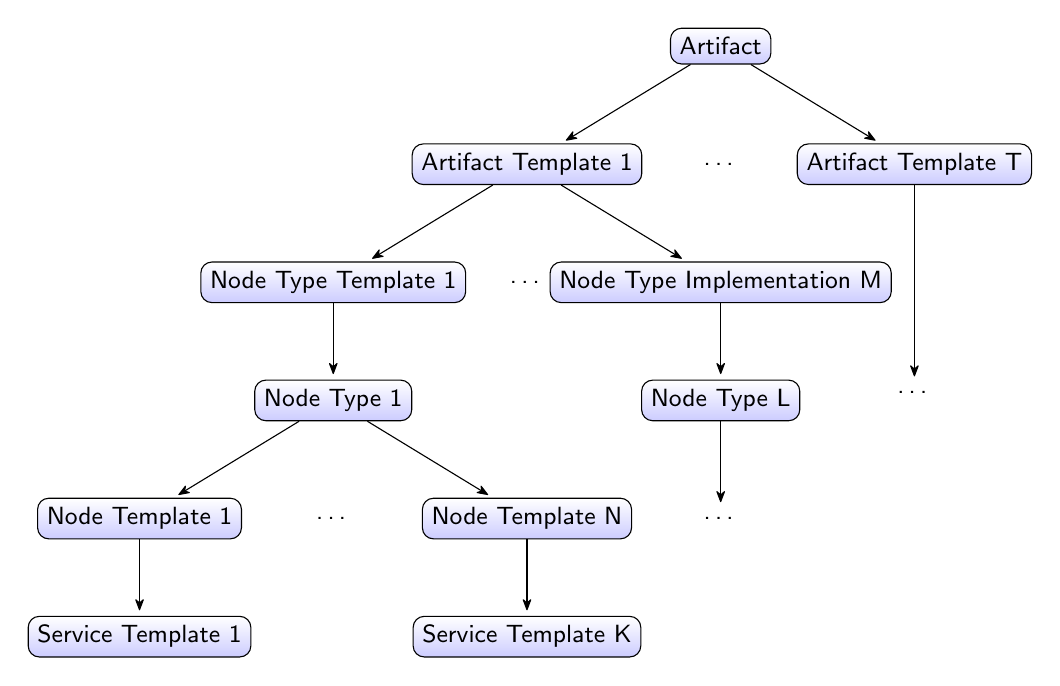
\begin{tikzpicture}[sibling distance=14em,->,>={Stealth[round,sep]},shorten >=1pt,auto,node distance=25mm]
    \node[main node] (1) {Artifact}
    child { node[main node](3) {Artifact Template 1} 
    	child { node[main node] (6) {Node Type Template 1} 
    			child { node[main node] (8) {Node Type 1} 
    				child { node[main node]  (11) {Node Template 1} 
    					child { node[main node] (13) {Service Template 1}}  
    				}
    				child { node[main node]  (12) {Node Template N} 
    					child { node[main node] (14) {Service Template K}}
    				}
    			}
    	}
    	child { node[main node] (7) {Node Type Implementation M} 
    		child { node[main node] (9) {Node Type L} 
    			child { node  (10) {\ldots} }
    		}
    	}
    }
    child { node[main node] (4) {Artifact Template T}  
    child { node (5) [below =of 4]{\ldots}}
	};

    \node at ($(3)!.5!(4)$) {\ldots};
    \node at ($(6)!.5!(7)$) {\ldots};
    \node at ($(11)!.5!(12)$) {\ldots};
    
\end{tikzpicture} 
\caption{An example tree describing how to find Service Templates and Node Templates for the given script} 	\label{fig:script_serv}
\end{figure}
Of course it is possible to move in opposite direction, starting from a Node and moving toward scripts, but this method brings additional complexity. 
Node Type can have several Node Type Implementations, but which one will be used can be determined only during deployment. 
The method presented above can uniquely determine Node Templates and Service Template for a given script.
Of course it is not guaranteed that found Node Type Implementation will be used during deployment, but we can't do anything with this. 
The following steps can be executed during a preprocessing, to identify necessary dependencies.
\begin{itemize}
	\item Find all Artifact Implementations to build dependency from script name to Artifact Implementation.
	\item Find all Node Type Implementation. Since those definitions contains both the Node Type and used Artifact Implementations, the dependency from script to Node Types can be build.
	\item Find all Service Templates, and in them contained Node Templates. So the necessary dependencies can be achieved (script to Node Template and script to Service Template).
\end{itemize}
\subsection*{Find external dependencies}
Analysis for external references.
Unfortunately it is impossible to identify all possible external dependencies, even within one language and one package manager (example in algorithm \ref{alg:unreadable}).
\begin{Algorithmus} 
	\caption{Unreadable bash script}
	\label{alg:unreadable}
	\begin{algorithmic}
		\State	\#!/bin/bash
		\State	$\textbf{set } line = $abcdefgijklmnoprst
		\State	$\textbf{set } word1 = \$\{line:0:1\}\$\{line:14:1\}\$\{line:17:1\}$ 
		\State  $\textbf{set } word2 = \$\{line:6:1\}\$\{line:4:1\}\$\{line:17:1\}$
		\State  $\$word1\$-\$word2\$$ install package
	\end{algorithmic}
\end{Algorithmus}
Since this work is aimed at creating a common tool that is easily expanded and supplemented, initially only basic usage of package managers will be considered, but complimented when necessary. 
Ease of adding modules to framework will proof correctness of architecture.
At the beginning, the most popular combination will be implemented, the $bash$ script with the $apt-get$ package manager.
This simple and powerful tool allows to install, delete or update the set of packages by writing one line.
When processing of this combination will reach an acceptable level, new languages and package managers will be added.
\subsection{Representing downloaded packages in TOSCA-Topology}
A package node denote to defined and instantiated element of \gls{tosca} topology, the purpose of which is to install the package.
The adding of new package nodes to TOSCA topology can be divided into several steps.
\begin{itemize}
	\item Add definitions for common elements, like artifacts or relations. This can be done once at preprocessing stage.
	\item The package node definition will be represented by a Node Type. There will be described that this node must be installed.
	\item Downloaded data and they installation script will be referenced by Artifact Template.
	\item Node Type Implementation will combine all artifacts.
	\item Node Template will instantiate a package in the corresponding Service Templates.
		To determine corresponding Service Template a preprocessing described in \nameref{subs:analyse} will be used.
	\item Reference Template will provide topology information, allowing the observer (user or runtime environment) to determine, for which nodes the package must be installed.
		References will be created both from origin Node Template to the package's Node Template and between Node Templates of created packages.
\end{itemize}
\subsection{Determining architecture of a final Platform}
The most acute way is the question about the architecture of the device where deployment scripts will be executed.
Unfortunately, it is impossible to analyze the structure of any CSAR and give an unambiguous answer to the question, on which architecture which command will be executed.
There are many pitfalls here.
A single Service Template can use several physical devices with different architectures.
The same Implementation Artifacts can refer to different Node Types, instantiated on different platforms.
So one simple Implementation Artifact with bash script containing "$apt$-$get$ $install$ $python$" command when deployed on different devices (for example with arm, amd64 and i386 architectures) will result in the loading and installation of 3 different packages. 
For an end user, the ability to use such a simple command is a huge relief, but for the framework it can greatly complicate analysis.
The following methods of architecture selection were designed.
\begin{itemize}
	\item Deployment environment analysis\\
	The script analyzing the system where it is running (for example using $uname$ $-a$ command) and depending on the result, installing the package corresponding to the architecture.
	\item Unified architecture\\
	An Unified architecture, predefined by the user at framework startup.
	\item Artifact specific architectures\\
	An architecture can be defined for each artifact.
\end{itemize}
\subsubsection*{Analysis of methods}
Unfortunately, the Deployment environment analysis, which at first glance seems to be the most reliable solution, brings many additional problems.
Packages for different platforms can differ not only by architecture, but also in the versions and the list of dependencies.
As a consequence, a complete chaos will be produced when trying to display these different packages with different versions in the \gls{tosca}-topology.
The only robust solution would be to create for each installed package a set of archives (one archive for each architecture), containing the entire dependency tree for the given package.
But this approach contradicts one of the ideas of this work: each package should be mapped in topology.\\
The Artifact specific architectures carries additional complexity to the user of the framework.
The user will be obligate to analyze each artifact and decide on which architecture it will be executed. 
This can be complicated by the fact that the same artifact can be executed on different architectures.\\
The method of the unified architecture was chosen, as the most simple and easy to implement.
If it will be necessary, this method can be easy expanded to Artifact specific architectures method (be replacing the user input to chose an unified architecture at start, by choosing an architecture for each artifact.) and to Deployment environment analysis (By downloading packages for all available architectures and adding the architecture determination to installation script.).

\subsection{Extensibility}
Framework should handle different script languages, each of them should support a various package managers.
This principle can be illustrated by a figure \ref{fig:lang_pm}.
% !TeX spellcheck = en_US

% We need layers to draw the block diagram
\usetikzlibrary{calc,positioning}

% Define a few styles and constants
\tikzstyle{entry}=[draw, fill=green!20, minimum height=2.0em, text width=8.0em]
\tikzstyle{ann} = [above, text width=5em]
\tikzstyle{framework} = [entry, text width=35em, fill=red!20, 
minimum height=19em, rounded corners]
\tikzstyle{lang} = [entry, text width=9em, fill=blue!20, 
minimum height=16em, rounded corners]
\def\blockdist{2.3}
\def\edgedist{2.5}

\begin{figure}
	\centering
\begin{tikzpicture}
\node (rr) [framework] {};
\node [xshift=+5mm, yshift=-2mm, below right] at (rr.north west) {\large References resolver framework };


\node (lang1) at ([xshift=-52mm,yshift=-4mm]rr) [lang] {};
\node [xshift=+3mm, yshift=-2mm, below right] at (lang1.north west) [text width=6em] {\large Language module 1 };
\node (lang2) at ([xshift=-7mm,yshift=-4mm]rr) [lang] {};
\node [xshift=+3mm, yshift=-2mm, below right] at (lang2.north west) [text width=6em] {\large Language module 2 };
\node (langn) at ([xshift=+52mm,yshift=-4mm]rr) [lang] {};
\node [xshift=+3mm, yshift=-2mm, below right] at (langn.north west) [text width=6em] {\large Language module N };  
\node at ($(lang2)!.5!(langn)$) {\ldots};

\node (l1pm1) at ([yshift=+15mm]lang1) [entry] {Package manager module};
\node (l1pm2) at ([yshift=0mm]lang1) [entry] {Package manager module};
\node (l1pmn) at ([yshift=-25mm]lang1) [entry] {Package manager module};
\node at ($(l1pm2)!.5!(l1pmn)$) {\vdots};

\node (l2pm1) at ([yshift=+15mm]lang2) [entry] {Package manager module};
\node (l2pm2) at ([yshift=0mm]lang2) [entry] {Download tool module};
\node (l2pm3) at ([yshift=-13mm]lang2) [entry] {Package manager module};
\node (l2pmn) at ([yshift=-25mm]lang2) [entry] {Package manager module};
%\node at ($(l2pm2)!.5!(l2pmn)$) {\vdots};

\node (lnpm1) at ([yshift=+15mm]langn) [entry] {Package manager module};
\node (lnpm2) at ([yshift=0mm]langn) [entry] {Package manager module};
\node (lnpm3) at ([yshift=-13mm]langn) [entry] {Download tool module};
\node (lnpmn) at ([yshift=-25mm]langn) [entry] {Download tool module};
%\node at ($(lnpm2)!.5!(lnpmn)$) {\vdots};


\end{tikzpicture} 
\caption{An example scheme representing several language modules containing package manager modules} 	\label{fig:lang_pm}
\end{figure}

\subsection{Result's checking}
Checking the results of the work is an important stage in the development of the program.
It is necessary to verify both the overall validity of the output \gls{csar}, and the possibility to deploy the output \gls{csar}.
To test for overall correctness, it is possible to use winery tool from OpenTOSCA.
This tool for creating and editing archives is also great for visualizing results.
Checking the deployment of the CSAR is a much more complicated task, for which OpenTOSCA runtime environment can be used. 
But it's also necessary to create proper environment for deploying the cloud application.

\section{Architecture}\label{sec:arch}
\if 0
Архитектура
В этом разделе будет описана архитектура фреймворка
Базовая концепция использования языков и обработчиков пакетов была представлена в главе ссылка на рисунке таком то, теперь опишем схему работы более подробно. 


\fi
\subsection{Preprocessing}
\if 0
В начале необходимо совершить процедуру предобработки для разархивации, добавления файлов и генерации зависимостей из пункта такого то
хорошим примером предобработки может послужить картинка такая то
картинка, на входе архив(облачком одна структура), на выходе -новая структура файлов с добавленными фаылами + зависимости

\fi
\subsection{Search for references}
\if 0
Как уже было указанно выше, модули языков анализируют каждый файл и проверяют его принадлежность к заданному языку, в случае принадлежности файлы передаются всем менеджерам пакетов данного языка. 
вставить картинку со стрелочками
В качестве примера можно привести следующую схему.
много разных фалов, язык баш отфильтровывает не скриптовые файлы, оставшийся поступает на анализ менеджеру пакетов апт-гет, который его изменяет и выдаёт на выходе имя пакета


\fi
\subsection{Package Handler}
\if 0
Следующий логический модуль - обработчик пакетов, по заданному имени пакета, он должен закгрузить сам пакет для установки, обратиться к менеджеру топологии для добавления пакета в топологию и рекурсивно повториться для каждой зависимости
картинка, не могу приудмать как это отобразить


\fi
\subsection{Topology Handler}
\if 0
Менеджер топологии получив имя пакета добавляет его в топологию тоски. выполнив пункты из обновления топологии тоски
отобразить его работу как генерацию новых файлов и обновление сервистэмплэйта
в завершение работы стоит добавить в схему зависимостей новую зависимость, новый тип для созданного пакета - во все сервис тэмплэйты его использующие


\fi
\subsection{Generalizing}
\if 0
В завершении необходимо упаковать все полученные результаты обратно в архив.

объединив все элементы инфраструктуры приложения,  получим следующую архитектуру
каринка с архитектурой, со всем элементами

след



\fi